%!TEX root = ../thesis.tex
\chapter{Conclusion and Outlook}
\label{ch:conclusion}

\section{Conclusion}

This thesis introduces a dataset with photos taken from hardware at the microbiology lab of FH Münster. Along with this an application for labeling is developed to make it quick and easy to create instance segmentation masks for colonies on plate images. 200 images are labeled with the help of the app. The app can be used continuously to increase the size of this dataset.

A Faster R-CNN model for object detection is trained on different configurations, with different combinations of data. Enhancing the created dataset with additional data yields a significant performance improvement. Other techniques for augmenting the dataset such as creating new images through the use of image generation models are explored but do not yield performance benefits.

Evaluating the best model from the experiments shows promising performance even for the small dataset size, and can be used to speed up the time-consuming counting process for plates by providing predictions that are correct approximately 8 out of 10 times while finding about 90\% of the colonies on an image.

\section{Outlook}

First of all, the model trained can be used via a simple web app as seen in Figure \ref{fig:detection_app}. The app is already deployed on a server at the FH Münster which performs the computation and can be accessed through a web browser on any device. So any photos taken with the photobox can be quickly counted with the help of the model.

\begin{figure}[hbt]
  \centering
  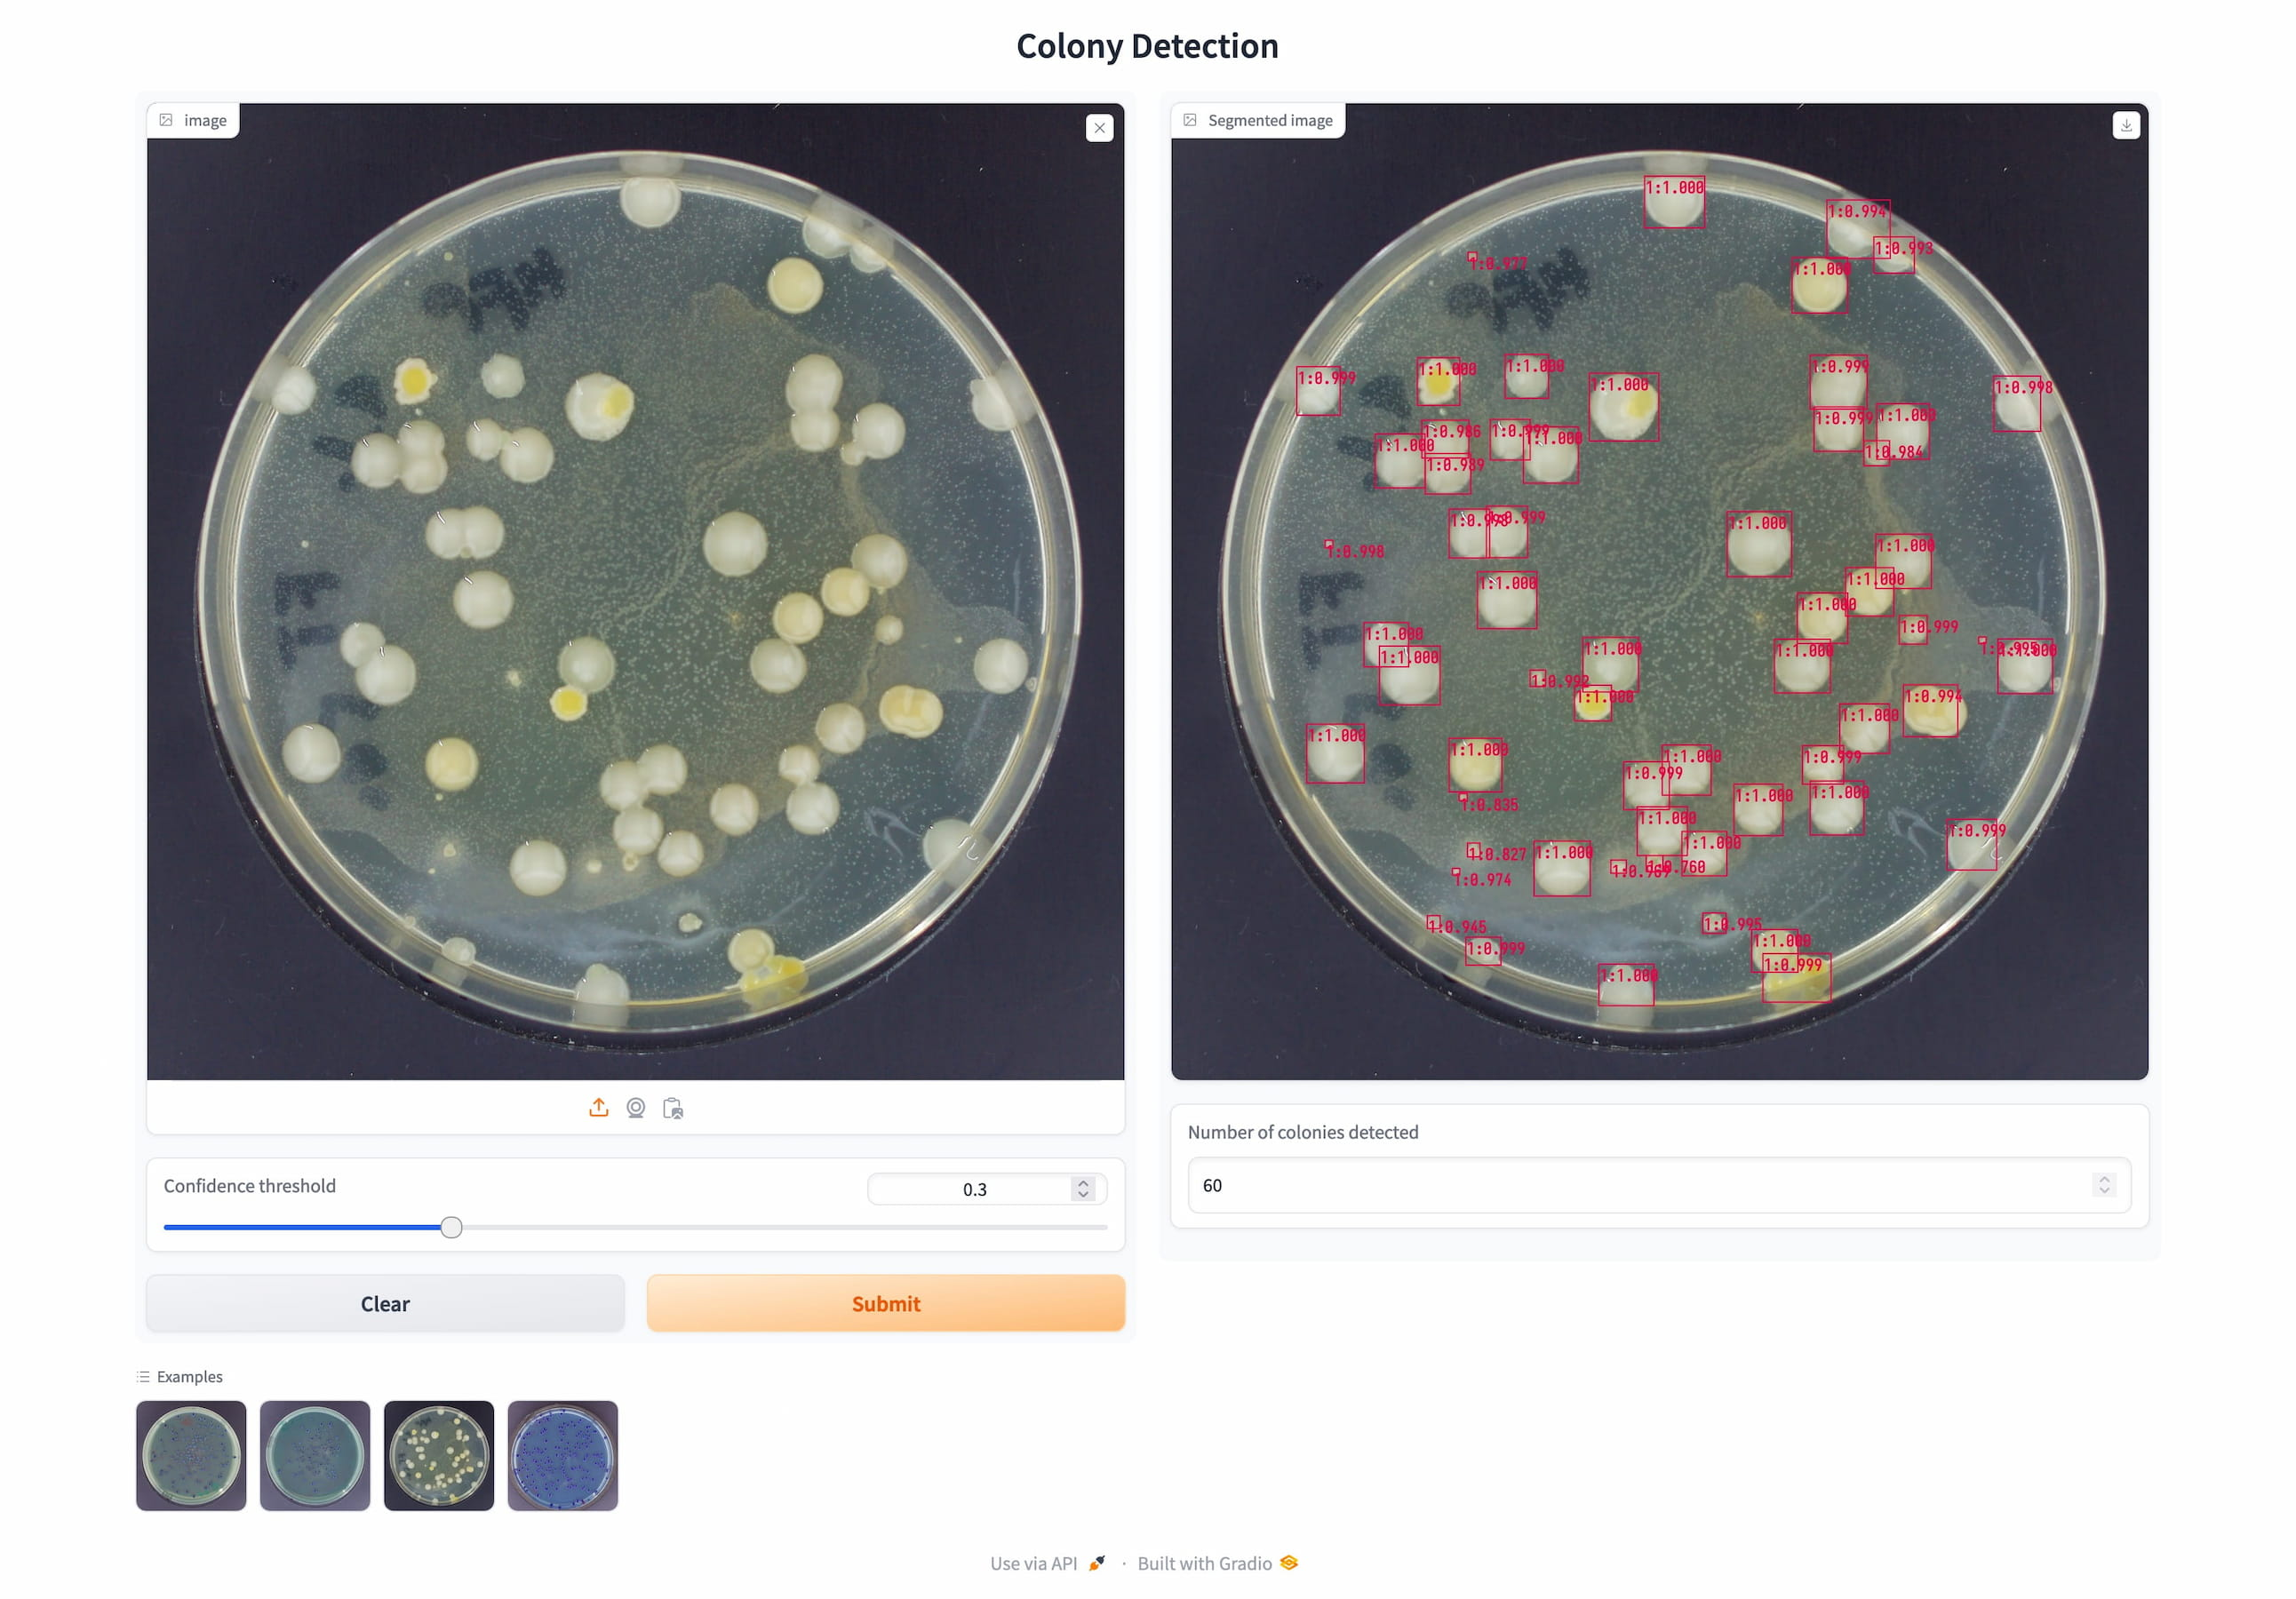
\includegraphics[width=0.8\textwidth]{assets/detection-app}
  \caption{Screenshot of the app used for detection}
  \label{fig:detection_app}
\end{figure}

One of the main areas for improvement is enlarging the dataset. It currently only holds 100 images for training and is biased towards certain image and colony types. This hurts general performance as previously shown. There are two main ways to increase the dataset size. 

First, the labeling tool introduced earlier can be used instead of counting by hand. This creates segmentation masks as a byproduct of counting colonies, which is a task that has to be performed frequently anyways.

The second opportunity for increasing the dataset size is to close the loop between inference and training. When using the model today for quick counting, it will sometimes make incorrect predictions which have to be corrected by a human. If these corrections are recorded, a new entry for the dataset could be created, ever improving the model performance.

This work focuses mostly on creating a suitable dataset and pipeline to create a great foundation for an automated detection system. Therefore only one model architecture, Faster R-CNN, was tested to prove that great detection on this task is attainable. It is possible that different model configurations or architectures perform better on this task. To squeeze more performance out of the existing dataset, it could prove useful to try out different model backbones or try out a single-shot object detection model like YOLOv4, which provided the best performance in \citet{Majchrowska_2022}.

Furthermore object detection architectures like Faster R-CNN support classification of objects, so it would be possible to not only locate colonies but also classify their species. For this, the dataset would have to be expanded by a classification layer, in addition to the segmentation masks.

And as a final remark, everything shown in here does not specifically rely on the photobox images. Smartphone cameras can also be used to capture the petri dish images, the labeling software can also be used in the same way for all types of images, and the model does not necessarily need high resolution images to reliably detect the colonies.

So in the future, students at the microbiology lab from FH Münster could take pictures of dishes using their smartphones, count the colonies using the help of the model developed here and the labeling app, which would feed back into the dataset and continuously improve the detection performance.
